\section{Appendix}
Combining CNNs and LSTMs (\autoref{fig:lstm-cnn-model}) offers several benefits. The LSTM+CNN model leverages
the strengths of both models, capturing both spatial features (through CNN) and
temporal dependencies (through LSTM) \cite{sainath2015convolutional}.
This makes them suitable for audio classification where temporal patterns are crucial.
This combination often leads to better performance in tasks that require understanding both
local features and global sequence patterns, such as speech recognition and music genre
classification. Moreover, LSTMs can handle variable-length sequences \cite{lim2020time},
making the combined model more flexible in processing audio segments of different lengths.

\vspace{-1em}
\begin{figure}[H]
  \centering
  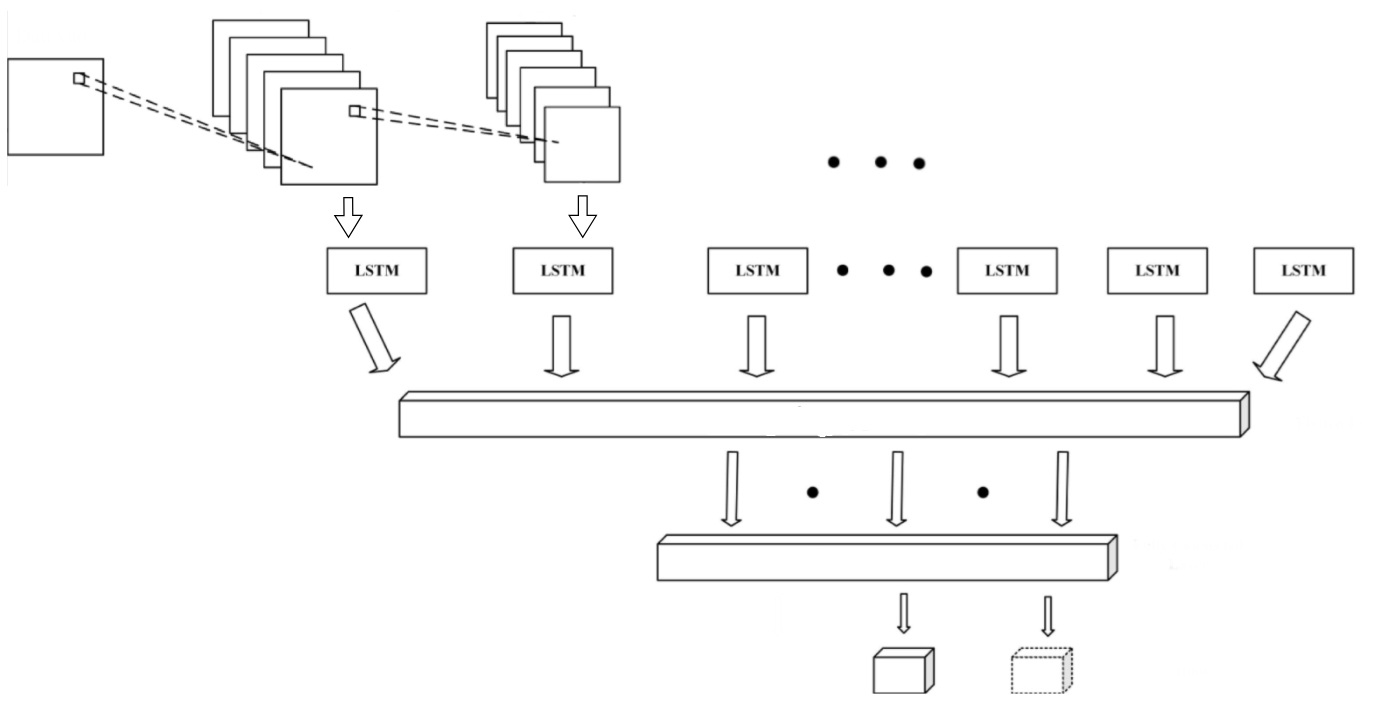
\includegraphics[width=0.47\textwidth]{LSTM-CNN-model.png}
  \caption{LSTM+CNN Model}
  \label{fig:lstm-cnn-model}
\end{figure}
\vspace{-1em}

However, combining CNNs and LSTMs results in more complex models with more parameters,
requiring more computational resources, and training LSTM+CNN models takes longer than
training a standalone CNN.
